% Real-robot setup (figure) and results (table) of Sec. 5.3, in ONE page-wide float so that the
% table always sits directly under the figure. Numbering is unaffected: the figure takes the next
% figure number, \captionof{table} the next table number.
%
% Efficiency, re-measured 2026-11-14 with the protocol of Table 1 (robot workstation, RTX 4090, batch 1,
% 5 input frames 480x640, 15x10 action chunk; T5 text encoding included; FLOPs counted as in Table 1,
% i.e. matmuls/convolutions incl. text encoder and VAE, attention-score FLOPs not counted):
%   Native : CUDA graphs for video DiT + action decoder     97.60 TFLOPs, median 1402.1 ms, 0.713 Hz
%   ARROW  : router + folded LoRA + graphed action decoder  49.25 TFLOPs, median  763.8 ms, 1.309 Hz
%   -49.5% FLOPs, 1.84x faster (2.06x without T5); per-task speedups 1.834-1.837x.
%   Stages (ms), T5 / video / action decoder: Native 161.5 / 892.1 / 351.2; ARROW 161.5 / 437.5 / 164.6.
%   Cross-check: Table 1(a) at 30% context (same 7,440 tokens) gives 98.0 -> 49.6 TFLOPs.
%   These numbers SUPERSEDE the first measurement (eager, live LoRA, no T5, FLOPs incl. attention:
%   154.5 -> 59.3 TFLOPs, mean 1257 -> 742 ms).
% Native + LoRA: first entered as an estimate (folded adapter = Native compute, 97.60 TFLOPs; latency
%   1402.1 x 704.0/701.7 = 1406.7 ms, 0.71 Hz); the author reported on 2026-11-14 that the measured
%   latency matches it, so the values stay as entered.
% SR (2026-11-14, author's sheet): successes out of 15 trials per task.
%   Sheet name   -> column            Native  Native+LoRA  ARROW
%   pick cup     -> Pick Cup from Sink   10       10        12
%   stack        -> Stack Bowls          12       12        14
%   pour water   -> Pour Water           11       12        12
%   open mic     -> Open Microwave        5        7        10
%   put cup      -> Cup out Microwave    10        9        13   (mapped by elimination; confirm)
%   open lid     -> Open Lid              6        7         9
%   Total                                54/90    57/90     70/90  -> Avg. 60.0 / 63.3 / 77.8
%   ARROW vs Native +17.8 pp (Fisher exact p = 0.015; task-stratified CMH p = 0.013);
%   ARROW vs Native + LoRA +14.4 pp (Fisher p = 0.049; CMH p = 0.046). Trials are not paired.
% Bold: best per column (Pour Water is a tie between Native + LoRA and ARROW).
\begin{figure*}[t]
  \centering
  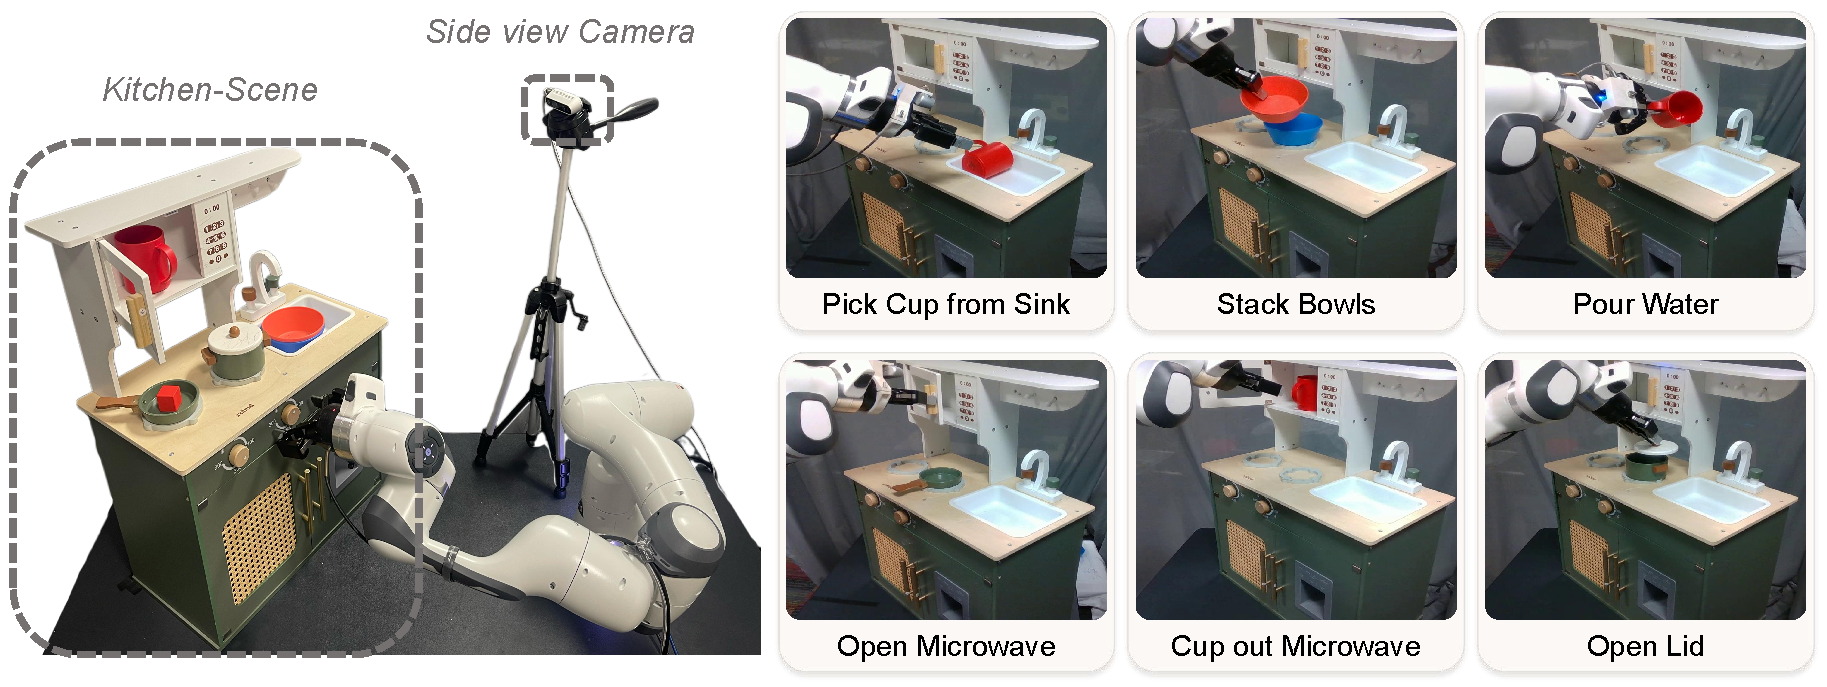
\includegraphics[width=0.8\textwidth]{robot_tasks_layout_cropped.pdf}
  \caption{\textbf{Real-robot environment and tasks.}
  Left: a Franka arm in a toy kitchen, recorded by a side-view camera.
  Right: the six evaluation tasks. \cj{XX one column? xx}}
  \label{fig:real_robot}

  \vspace{8pt}

  \definecolor{ArrowOurs}{HTML}{EBE9FF}
  \captionof{table}{\textbf{Real-robot results of mimic-video.}
  Success rate (SR, \%) over 15 trials per task; Avg.: mean over the six tasks.
  Lat.: median latency per query on an RTX 4090 at batch size one, including text encoding; Freq.: $1/$Lat.
  Deployment settings follow \cref{tab:main_results}.
  FLOPs are counted as in \cref{tab:main_results}, including text encoding and the VAE.
  \method keeps 7,440 of the 19,200 context tokens.
  Bold: best per column; lavender: \method.}
  \label{tab:real_robot}
  \footnotesize
  \setlength{\tabcolsep}{2.5pt}
  \renewcommand{\arraystretch}{1.1}
  \begin{tabularx}{\textwidth}{@{}>{\raggedright\arraybackslash}p{1.9cm}*{10}{>{\centering\arraybackslash}X}@{}}
    \toprule[1pt]
    & \multicolumn{7}{c}{SR (\%) $\uparrow$} & \multicolumn{3}{c}{Efficiency} \\
    \cmidrule(lr){2-8}\cmidrule(l){9-11}
    Method
      & \makecell{Pick Cup\\from Sink} & \makecell{Stack\\Bowls} & \makecell{Pour\\Water}
      & \makecell{Open\\Microwave} & \makecell{Cup out\\Microwave} & \makecell{Open\\Lid} & Avg.
      & \makecell{Freq.\\(Hz) $\uparrow$} & \makecell{Lat.\\(ms) $\downarrow$} & \makecell{FLOPs\\(T) $\downarrow$} \\
    \midrule
    Native
      & 66.7 & 80.0 & 73.3 & 33.3 & 66.7 & 40.0 & 60.0
      & 0.71 & 1402.1 & 97.60 \\
    Native + LoRA
      & 66.7 & 80.0 & \textbf{80.0} & 46.7 & 60.0 & 46.7 & 63.3
      & 0.71 & 1406.7 & 97.60 \\
    \rowcolor{ArrowOurs}
    \method
      & \textbf{80.0} & \textbf{93.3} & \textbf{80.0} & \textbf{66.7} & \textbf{86.7} & \textbf{60.0} & \textbf{77.8}
      & \textbf{1.31} & \textbf{763.8} & \textbf{49.25} \\
    \bottomrule[1pt]
  \end{tabularx}
\end{figure*}
